%
%                  Politecnico di Milano
%
%         Student: Caravano Andrea, Alberto Cantele
%            A.Y.: 2024/2025
%
%   Last modified: 19/03/2025
%
%     Description: Internet of Things: Challenge n. 1
%                  Theoretical exercise
%

\documentclass[a4paper,11pt]{article} % tipo di documento
\usepackage[T1]{fontenc} % codifica dei font
\usepackage[utf8]{inputenc} % lettere accentate da tastiera
\usepackage[english,italian]{babel} % lingua del documento
\usepackage{lipsum} % genera testo fittizio
\usepackage{url} % per scrivere gli indirizzi Internet e/o di riferimento nella pagina

\usepackage[hidelinks]{hyperref} % per modificare il comportamento dei collegamenti ipertestuali (+ leva colore attorno)

\usepackage[margin=0.7in]{geometry} % margine di pagina

\usepackage{graphicx} % per inserire immagini

\usepackage[outputdir=../auxil]{minted} % per colorazione automatica del codice (installare pygments da Homebrew)
% \usepackage{pythonhighlight} % per Python

\setminted{ % si può impostare il linguaggio specifico con \setminted[JSON] ad esempio
    linenos=true,
    breaklines=true,
    encoding=utf8,
    fontsize=\normalsize,
    frame=lines
}

\usepackage{fancyhdr}
\usepackage{textcomp}
\usepackage{siunitx} % per gestione intestazione e piè di pagina

\usepackage{tcolorbox} % per riquadrature di vario colore

\hypersetup{ % metadati di titolo e autore nel PDF
    pdftitle={Internet of Things: Challenge n. 1},
    pdfauthor={Andrea Caravano, Alberto Cantele}
}

\setlength{\parindent}{0pt} % rimuove l'indentazione del testo

\tcbset{ % impostazioni per riquadrature
    colback=gray!20,
    colframe=black,
    boxrule=0.5pt
}

\begin{document}
    \pagestyle{fancy}
    \fancyhead{}\fancyfoot{}
    \fancyhead[L]{\textbf{Internet of Things: Challenge n. 1}}
    \fancyhead[R]{Andrea Caravano, Alberto Cantele}
    \fancyfoot[C]{\thepage}

    \title{\textbf{Internet of Things}\\Challenge n. 1: Theoretical exercise}
    \author{Andrea Caravano, Alberto Cantele}
    \date{Academic Year 2024--25}
    \maketitle


    \section{Exercise text}\label{sec:exercise-text}
    In the parking lot, there are 10 sensors that monitor the parking spaces.

    Each sensor has a fixed position (x, y) in the parking lot reported in Table.

    \begin{center}
        \begin{tabular}{|c|c|}
            \hline
            Sensor & Coordinates (x, y) \\
            \hline
            1      & (1, 2)             \\
            \hline
            2      & (10, 3)            \\
            \hline
            3      & (4, 8)             \\
            \hline
            4      & (15, 7)            \\
            \hline
            5      & (6, 1)             \\
            \hline
            6      & (9, 12)            \\
            \hline
            7      & (14, 4)            \\
            \hline
            8      & (3, 10)            \\
            \hline
            9      & (7, 7)             \\
            \hline
            10     & (12, 14)           \\
            \hline
        \end{tabular}
    \end{center}

    \begin{center}
        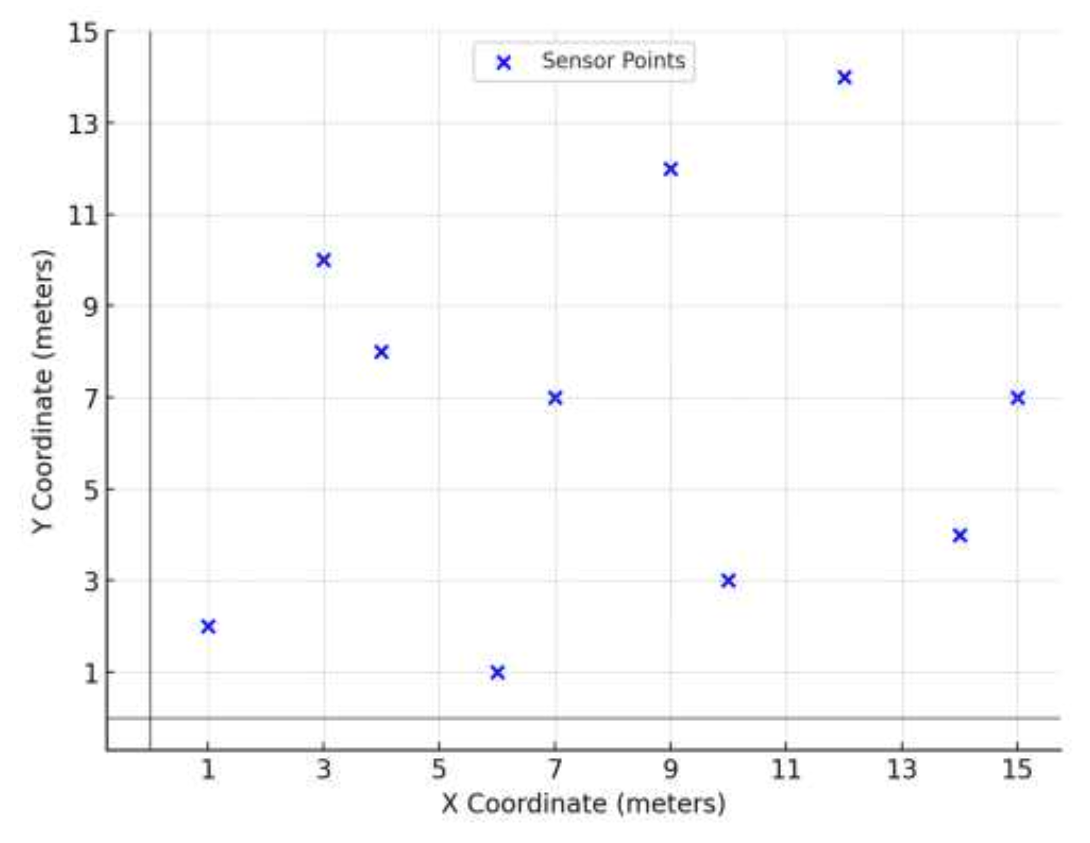
\includegraphics[width=10cm]{../res/sensor_nodes}
    \end{center}

    \begin{itemize}
        \item Each sensor transmits a status update every 10 minutes.
        \item The packet size is $b = 2000$ bit, and the initial energy per sensor is $E_b = 5$ mJ\@.
        \item The energy consumption for transmission depends on the distance between the sensor and the sink:
        \begin{itemize}
            \item Energy for the TX/RX circuitry: $E_c = 50$ nJ/bit
            \item Energy for transmission: $E_{tx}$(d) = k \cdot $d^2$ nJ/bit, where d is the distance from the sensor to the sink, and $k = 1$ nJ/bit/$m^2$
        \end{itemize}
    \end{itemize}

    \begin{enumerate}
        \item Find the lifetime of the system when the sink is placed at the fixed position ($x_s$, $y_s$) = (20, 20).

        The lifetime is defined as the time until the first sensor's battery dies, based on the energy consumption of the sensors.
        \item Find the optimal position of the sink that maximizes the system lifetime.

        Provide the coordinates ($x_s$, $y_s$) of the sink that minimizes the energy consumption of the worst-case sensor (the sensor that consumes the most energy).
        \item Discuss the trade-offs involved in choosing a fixed sink position versus dynamically moving the sink.

        Consider the impact on system lifetime and energy consumption of each sensor.
    \end{enumerate}

    Let's tackle each point singularly.


    \section{Lifetime of the system with a fixed sink position}\label{sec:lifetime-of-the-system-with-a-fixed-sink-position}

    This part of the exercise can be solved by hand using the same approach seen during the theoretical exercise sessions.

    In particular, part of the intuition to save up some time in the computation is determining the furthest-distanced node, given the sink position.

    Just upon observation of the diagram, the matching sensor would be the first.

    A sketch of the solution is provided in the following.

    \subsection{Solution sketch}\label{subsec:solution-sketch}

    Data declaration:

    \medskip

    Given the set of coordinates

    Status Update Period (SU) = $10 \cdot 60$ seconds

    Packet size ($P_s$) = 2000 bits

    Energy budget ($E_b$) = $5 \cdot 10^{-3}$ Joule

    Energy for operating the circuitry ($E_c$) = $50 \cdot 10^{-9}$ Joule/bit

    Energy for transmission ($E_{tx}$(d)) = k \cdot $d^2$ J/bit, where d is the distance from the sensor to the sink

    K constant ($k$) = $1 \cdot 10^{-9}$ J/bit/$m^2$

    Sink (constant) = $(20, 20)$

    \bigskip

    A fixed value among all sensors is the energy for operating the circuitry for each packet (the minimum transmission unit, of course):

    $E_{c per packet}$ = $E_c \cdot P_s$ = $50 \cdot 10^{-9} \cdot 2000$ = $0,1$ mJ/packet

    \bigskip

    Let's now compute the Euclidean distance from the sink to the first node position:

    \smallskip

    $d = \sqrt{{(x_s - x_1)}^2+{(y_s - y_1)}^2} = \sqrt{{(20 - 1)}^2+{(20 - 2)}^2}$ \simeq 26,17

    \bigskip

    The only missing piece now is the energy needed for transmission:

    \smallskip

    $E_{tx}(d) = k \cdot d^2 = 1 \cdot 10^{-9} \cdot (26,17)^2 = 685$ nJ/bit

    \smallskip

    That, per each packet, translates to:

    \smallskip

    $E_{tx per packet}(d) = E_{tx}(d) \cdot P_s = 685 \cdot 10^{-9} \cdot 2000 = 1,37$ mJ/packet

    \smallskip

    And results, in the end, to a total sensor consumption of:

    \smallskip

    $E_1 = E_{c per packet} + E_{tx per packet} = 0,1$ mJ $+ 1,37$ mJ $= 1,47$ mJ/packet

    \bigskip

    With a matching lifetime of:

    \smallskip

    $L_1 = \lfloor \frac{E_b}{E_1} \rfloor = 3$ cycles $= 3 \cdot SU = 3 \cdot 10 \cdot 60$ seconds $= 1800$ seconds $= 30$ minutes

    \subsection{Automation via code (Python)}\label{subsec:automation-via-code-(python)}

    This solution pattern has been replicated for all sensor nodes using a small Python script, confirming the expected theoretical results.

    The resulting output is shown in the following, while the code is provided in the \hyperref[subsec:lifetime-of-the-system-with-a-fixed-sink-position]{final section of the document}.

    \begin{tcolorbox}
        Sensor node n. 1 - energy per packet: 1.47 mJ - lifetime: 3 cycles = 30.0 minutes

        Sensor node n. 2 - energy per packet: 0.878 mJ - lifetime: 5 cycles = 50.0 minutes

        Sensor node n. 3 - energy per packet: 0.9 mJ - lifetime: 5 cycles = 50.0 minutes

        Sensor node n. 4 - energy per packet: 0.488 mJ - lifetime: 10 cycles = 100.0 minutes

        Sensor node n. 5 - energy per packet: 1.214 mJ - lifetime: 4 cycles = 40.0 minutes

        Sensor node n. 6 - energy per packet: 0.47 mJ - lifetime: 10 cycles = 100.0 minutes

        Sensor node n. 7 - energy per packet: 0.684 mJ - lifetime: 7 cycles = 70.0 minutes

        Sensor node n. 8 - energy per packet: 0.878 mJ - lifetime: 5 cycles = 50.0 minutes

        Sensor node n. 9 - energy per packet: 0.776 mJ - lifetime: 6 cycles = 60.0 minutes

        Sensor node n. 10 - energy per packet: 0.3 mJ - lifetime: 16 cycles = 160.0 minutes

        \medskip

        The sensor node with the worst lifetime is the sensor n. 1 which has a lifetime of 3 cycles = 30.0 minutes and energy per packet of 1.47 mJ
    \end{tcolorbox}


    \section{Optimization problem: the best position for the sink node}\label{sec:optimization-problem:-the-best-position-for-the-sink-node}

    \subsection{Solution sketch}\label{subsec:solution-sketch2}

    A resolution algorithm is described by the following procedural steps, that mimic an operational research problem solution, in closed form.

    \begin{itemize}
        \item Boundaries of the inspection are defined as the minimum and maximum vertical and horizontal position.

        Of course, no solution could yield a better result outside of this research scope, as they would only increase the distance.
        \item Final result variables are prepared for the research of the best energy consumption.
        \item A loop is organized on all possible sink positions, with a step of 0.1.

        Further optimizations could use a higher step, depending on the correspondence to the real-world positioning.
        \item Per each candidate sink position, the most distant node is detected among all sensors.

        This is the one providing the worst energy consumption result, as \hyperref[subsec:solution-sketch]{demonstrated in the first part of the exercise}.
        \item The same computation \hyperref[subsec:solution-sketch]{explained in the first part} is replicated, determining the best-performing energy figure per packet (therefore, consuming less energy).
        \item Upon detection of a new best minimum, temporary lowest energy per packet and determined lifetime, corresponding to the sink used for computation, are stored.
        \item At the end of the cycle, we have finally determined the best sink coordinates and their energy consumption and lifetime, that are shown in output.
    \end{itemize}

    The algorithm is therefore iteratively searching for the best energy consumption (so, the lowest one) among all the most distant sensor nodes from a given sink node.

    The sink node providing the best energy-consuming sensor node is the winner.

    \subsection{Automation via code (Python)}\label{subsec:automation-via-code-(python)2}

    This solution pattern has been implemented using a small Python script.

    The resulting output is shown in the following, while the code is provided in the \hyperref[subsec:lifetime-of-the-system-with-a-fixed-sink-position]{final section of the document}.

    \begin{tcolorbox}
        Determining the best sink position in the close form (x: (1 -> 15), y: (1 -> 14))

        \smallskip

        The best sink position determined in the close form is (x, y) = (6.9, 7.6),

        \smallskip

        with the worst-performing energy-wise node having consumption of 0.23 mJ, corresponding to a lifetime of 21 cycles
    \end{tcolorbox}


    \section{Sink position: static vs dynamic}\label{sec:sink-position:-static-vs-dynamic}

    As we noticed approaching the first part of the exercise, distancing of the sensor node with respect to the sink node plays a fundamental role in determining its energy consumption figure (and, therefore, lifetime).

    Accordingly, a careful planning of the sink positioning can hugely impact on the battery maintenance cycle and reduce the need for replacements over time.

    Let's discuss the design trade-off in both the static fixed position approach versus the dynamically determined one.

    \subsection{Static positioning}\label{subsec:static-positioning}

    \subsubsection{Load balancing}

    In a balanced environment, all sensor nodes are, mostly, equally employed and the occupancy state detection job is shared among all sensor nodes, that will therefore need to transmit updates to the sink node with a sensibly similar frequency.

    This is the case, for example, in which a supermarket's parking lot falls in, during opening hours: customers are entering and exiting their slot with a mostly regular frequency.

    Overnight, instead, the parking lot is expected to be empty: as a result, the frequency of updates of sensor nodes will still be similar among them.

    This is the perfect example in which the usage of a statically placed sink node is the best approach.

    With careful and preventive planning, like the one we discussed in the second point of the exercise, we are able to minimize the power consumption of each sensor up to the most reasonable limit, providing equal fairness to all nodes.

    \subsubsection{Planned load imbalance}

    If, instead, nodes are not expected to provide equal usage figures, it is inconvenient to maintain the same positioning strategy as the one applied assuming equally distributed load among nodes.

    The case in which a group of sensor nodes is more heavily used than another one should be taken into consideration.

    Let's imagine that sensors 3, 8 and 9 produces the great majority of updates: this may be due to real-world conditions of the parking slot (for example, they may be the only free parking slot, while the others require the payment of an access fee).

    The most reasonable place to put the sink would be located into a favourable position for this group of sensors rather than the other ones.

    \subsection{Dynamic positioning}\label{subsec:dynamic-positioning}

    \subsubsection{Dynamic load imbalance}

    Let's now assume that the group of heavily employed nodes changes over the evolution of the system.

    This is the case in which, for example, a big parking lot is divided in different areas and some of them are more visited than other ones, during a promotional event, creating a peak of visitors.

    Dynamic placement of the sink node is therefore ideal in a dynamic load imbalance setting.

    \subsubsection{Movements consume energy}

    In a dynamic load imbalancing scenario, assuming a human-moved sink node is unrealistic, as it would probably come at a higher cost than the disadvantage of a poorly placed sink node.

    Therefore, we should consider an added energy consumption term due to the movement of the sink node during the system's evolution and also add it to the trade-off evaluation.

    \subsubsection{A distributed system}

    The implementation of a distributed sink comes as a cost for both the physical devices and overhead in synchronization and replication among the distributed nodes of a global sink node.

    However, it is directly pointed at exploiting the nearest distributed sink node when sending updates (and also, add reliability on top of that).

    The usage peak mentioned in the example above would, in fact, benefit from the presence of a distributed sink node near to the group of sensors covering a parking area by minimizing their energy consumption estimation, overall.


    \section{Code solution sketch}\label{sec:code-solution-sketch}

    \subsection{Lifetime of the system with a fixed sink position}\label{subsec:lifetime-of-the-system-with-a-fixed-sink-position}

    \begin{minted}{Python}
import math
import numpy as np
import sys

# Prepare problem data
coordinates = [
    [1, 2],
    [10, 3],
    [4, 8],
    [15, 7],
    [6, 1],
    [9, 12],
    [14, 4],
    [3, 10],
    [7, 7],
    [12, 14],
]  # meters

status_update_period = 10 * 60  # 10 minutes, expressed in seconds
packet_size = 2000  # bits
energy_budget = 5 * 10 ** (-3)  # Joule
energy_circuitry = 50 * 10 ** (-9)  # Joule
k_transmission = 1 * 10 ** (-9)  # J/bit/m^2
sink = [20, 20]  # meters

# Fixed value: energy required to operate the TX/RX circuitry, as it does not depend on distance
ec_per_packet = energy_circuitry * packet_size

energies = []
lifetimes = []
for i in range(0, len(coordinates)):
    # Euclidean distance computation ("diagonally") from the sender to the sink node
    distance = math.sqrt(
        (sink[0] - coordinates[i][0]) ** 2 + (sink[1] - coordinates[i][1]) ** 2
    )
    # Energy for transmission per each packet
    etx_per_packet = k_transmission * distance**2 * packet_size
    # Total energy per packet
    energy_per_packet = ec_per_packet + etx_per_packet
    energies.append(energy_per_packet)
    # Let's now compute how many packets (duty cycles, as one per duty cycle is sent) fit in the energy budget
    lifetime = math.floor(energy_budget / energy_per_packet)
    lifetimes.append(lifetime)
    print(
        "Sensor node n. "
        + str(i + 1)
        + " - energy per packet: "
        + str(round(energy_per_packet * 10**3, 3))
        + " mJ - lifetime: "
        + str(lifetime)
        + " cycles = "
        + str(lifetime * status_update_period / 60)
        + " minutes"
    )

# Let's now compute the index of the sensor node that had the worst lifetime!
index_worst = np.argmax(lifetime)
print(
    "\n\nThe sensor node with the worst lifetime is the sensor n. "
    + str(index_worst + 1)
    + " which has a lifetime of "
    + str(lifetimes[index_worst])
    + " cycles = "
    + str(lifetimes[index_worst] * status_update_period / 60)
    + " minutes and energy per packet of "
    + str(round(energies[index_worst] * 10**3, 3))
    + " mJ"
)
    \end{minted}

    \subsection{Optimization problem: the best sink position for the sink node}\label{subsec:optimization-problem:-the-best-sink-position-for-the-sink-node}

    \begin{minted}{Python}
# Constants
MARGIN = 0  # Added margin, to let sink exploration reach the maximum reasonable limit, even if no better results are expected trespassing the boundaries
SINK_MIN_HORIZONTAL = max(
    # Minimum value of the horizontal component of coordinates
    min(coord[0] for coord in coordinates) - MARGIN,
    0,  # Coordinates start from 0, so if the minimum coordinate - the additive component results to be less than 0, we put a fixed limit at 0, of course
)
SINK_MAX_HORIZONTAL = max(coord[0] for coord in coordinates) + MARGIN
SINK_MIN_VERTICAL = max(min(coord[1] for coord in coordinates) - MARGIN, 0)
SINK_MAX_VERTICAL = max(coord[1] for coord in coordinates) + MARGIN

# Final result
lowest_energy_per_packet = sys.float_info.max
optimized_lifetime = None
best_sink = [None, None]

print(
    "Determining the best sink position in the close form (x: (%d -> %d), y: (%d -> %d))"
    % (SINK_MIN_HORIZONTAL, SINK_MAX_HORIZONTAL, SINK_MIN_VERTICAL, SINK_MAX_VERTICAL)
)
# Loop steps of 0.1 (more than that seems unreasonable in a real-world setting)
for i in np.arange(SINK_MIN_HORIZONTAL, SINK_MAX_HORIZONTAL + 0.1, 0.1):
    for j in np.arange(SINK_MIN_VERTICAL, SINK_MAX_VERTICAL + 0.1, 0.1):
        # Temporary sink position
        sink = [i, j]
        # This will contain the set of distances from each sensor to the new temporary sink node
        distance_set = []
        # Again, iterate over each sensor computing the distance
        for k in range(0, len(coordinates)):
            # Euclidean distance computation ("diagonally") from the sender to the sink node
            distance = math.sqrt(
                (sink[0] - coordinates[k][0]) ** 2 + (sink[1] - coordinates[k][1]) ** 2
            )
            # And add it to the local set
            distance_set.append(distance)

        # Energy for transmission per each packet
        etx_per_packet = k_transmission * max(distance_set) ** 2 * packet_size
        # Total energy per packet
        energy_per_packet = ec_per_packet + etx_per_packet
        # Let's now compute how many packets (duty cycles, as one per duty cycle is sent) fit in the energy budget
        lifetime = math.floor(energy_budget / energy_per_packet)
        # Classical minimum energy computation
        if energy_per_packet < lowest_energy_per_packet:
            # The resulting best energy consumption and lifetime values
            lowest_energy_per_packet = energy_per_packet
            optimized_lifetime = lifetime
            # And therefore the sink position is registered as the temporary best
            best_sink = sink

# The result has been finally determinated
print(
    "The best sink position determined in the close form is (x, y) = (%.1f, %.1f), \nwith the worst-performing energy-wise node having consumption of %.2f mJ, corresponding to a lifetime of %d cycles"
    % (best_sink[0], best_sink[1], lowest_energy_per_packet * 10**3, optimized_lifetime)
)
    \end{minted}
\end{document}
